\documentclass[11pt,a4paper]{article}

% Packages
\usepackage[margin=1in]{geometry}
\usepackage{hyperref}
\usepackage{parskip} % adds space between paragraphs
\usepackage{enumitem} % for better lists
\usepackage{tikz} % for diagrams
\usepackage{xcolor} % for colored boxes in tikz

% Hyperlinks color
\hypersetup{
    colorlinks=true,
    linkcolor=blue,
    urlcolor=blue
}

\begin{document}

%==========================
% Title & Author
%==========================
\begin{center}
    {\LARGE \textbf{Modeling Human Attention Across Modalities, Content Features, and Algorithmic Exposure}}\\[2mm]
    {\large Khadidiatou Cissé, MSc Mathematics - Performance Engineering - Data \& ML Research} \\[1mm]
    GitHub: \href{https://github.com/Khadiijatu}{github.com/Khadiijatu} \quad • \quad LinkedIn: \href{https://www.linkedin.com/in/khadijatea}{linkedin.com/in/khadijatea} \\[1mm]
    \textbf{Status:} Ongoing independent research project. Manuscript in preparation.
\end{center}

\vspace{5mm}

%==========================
% Overview / Motivation
%==========================
\section*{Overview \& Motivation}
Human attention is a central concept in cognition, learning, and digital interactions.  
However, most studies rely on coarse engagement metrics and do not integrate content structure, modality, and algorithmic context.  

This project investigates attention as an observable, structured signal arising from the interaction between content features, modality, and recommendation algorithms.  
The focus is on \textbf{interpretability, rigorous quantitative modeling, and reproducibility}.

%==========================
% Schematic Diagram
%==========================
\section*{Conceptual Diagram}
\begin{center}
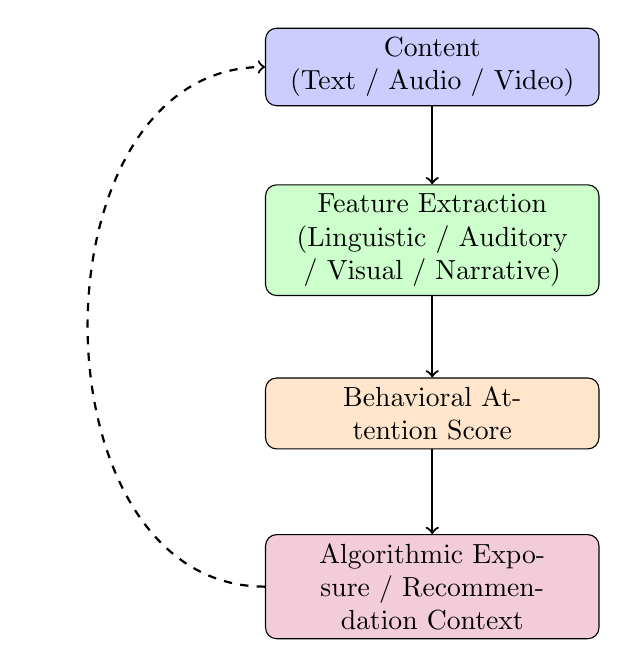
\begin{tikzpicture}[node distance=2.2cm, auto]

% Nodes
\node[draw, rectangle, rounded corners, fill=blue!20, text width=4cm, align=center] (content) {Content \\ (Text / Audio / Video)};
\node[draw, rectangle, rounded corners, fill=green!20, text width=4cm, align=center, below of=content] (features) {Feature Extraction \\ (Linguistic / Auditory / Visual / Narrative)};
\node[draw, rectangle, rounded corners, fill=orange!20, text width=4cm, align=center, below of=features] (attention) {Behavioral Attention Score};
\node[draw, rectangle, rounded corners, fill=purple!20, text width=4cm, align=center, below of=attention] (algo) {Algorithmic Exposure / Recommendation Context};

% Arrows
\draw[->, thick] (content) -- (features);
\draw[->, thick] (features) -- (attention);
\draw[->, thick] (attention) -- (algo);

% Feedback loop (optional)
\draw[->, thick, dashed] (algo.west) .. controls +(-3,0) and +(-3,0) .. (content.west);

\end{tikzpicture}
\end{center}

%==========================
% Research Questions
%==========================
\section*{Research Questions}
\begin{enumerate}[leftmargin=*]
    \item How does attention vary across content modalities (text, audio, video) for different topics?
    \item Which content features (linguistic, auditory, visual, narrative) are most strongly associated with attention?
    \item How does algorithmic exposure (recommended vs non-recommended content) interact with features?
    \item Are multiple distinct feature configurations capable of eliciting high attention?
\end{enumerate}

%==========================
% Dataset Design & Attention Score
%==========================
\section*{Dataset Design \& Attention Score}
\begin{itemize}[leftmargin=*]
    \item Content is sampled across multiple platforms and domains: lifestyle, mental health, science, technology, culture, art, environment, education.
    \item Modalities: text, audio, video
    \item Algorithmic exposure annotated as \textit{recommended} vs \textit{non-recommended} based on observable platform signals.
    \item \textbf{Behavioral attention score} combines normalized engagement proxies: dwell time, completion rate, replay/revisit signals, interaction-adjusted engagement.
    \item Score is modality-aware and normalized for content length. Interpreted as a proxy for behavioral attention, not neural attention.
\end{itemize}

%==========================
% Feature Extraction
%==========================
\section*{Feature Extraction}
\begin{itemize}[leftmargin=*]
    \item \textbf{Linguistic:} text length, lexical diversity, sentence/paragraph structure, readability metrics
    \item \textbf{Auditory:} speech rate, pitch variability, pauses, background music/sounds
    \item \textbf{Visual:} motion intensity, color dynamics, visual complexity, cuts/scene changes
    \item \textbf{Structural/Narrative:} pacing, segmentation, storytelling markers, conversational indicators
\end{itemize}

%==========================
% Modeling Strategy
%==========================
\section*{Modeling Strategy}
\begin{itemize}[leftmargin=*]
    \item Mixed-effects models to account for topic and creator variability
    \item Feature-group comparisons for explanatory power
    \item Unsupervised clustering to identify distinct attention profiles
    \item Selective nonlinear modeling for theoretically motivated features
    \item Emphasis on \textbf{interpretability over prediction}
\end{itemize}

%==========================
% Expected Contributions
%==========================
\section*{Expected Contributions}
\begin{itemize}[leftmargin=*]
    \item Unified framework for attention modeling across modalities
    \item Feature-based understanding of attention patterns
    \item Foundation for studying content–algorithm–attention feedback loops
    \item Basis for future alignment with neural/physiological measures (EEG, eye-tracking)
\end{itemize}

%==========================
% Limitations & Future Directions
%==========================
\section*{Limitations \& Future Directions}
\begin{itemize}[leftmargin=*]
    \item Observational data only; no causal claims
    \item Platform-dependent attention proxies
    \item Behavioral attention is an approximation of cognitive attention
    \item Future extensions: integrate brain/physiological data, explore category-theory or other abstract models of attention dynamics, expand to cross-cultural datasets
\end{itemize}

\end{document}
